% Thank you Josh Davis for this template!
% https://github.com/jdavis/latex-homework-template/blob/master/homework.tex

\documentclass{article}

% ----------

% Packages

\usepackage{fancyhdr}
\usepackage{extramarks}
\usepackage{amsmath}
\usepackage{amssymb}
\usepackage{amsthm}
\usepackage{amsfonts}
\usepackage{tikz}
\usepackage[plain]{algorithm}
\usepackage{algpseudocode}
\usepackage{enumitem}
\usepackage{chngcntr}

% Libraries

\usetikzlibrary{automata, positioning, arrows}

%
% Basic Document Settings
%

\topmargin=-0.45in
\evensidemargin=0in
\oddsidemargin=0in
\textwidth=6.5in
\textheight=9.0in
\headsep=0.25in

\linespread{1.1}

\pagestyle{fancy}
\lhead{\hmwkAuthorName}
\chead{}
\rhead{\hmwkClass\ (\hmwkClassInstructor): \hmwkTitle}
\lfoot{\lastxmark}
\cfoot{\thepage}

\renewcommand\headrulewidth{0.4pt}
\renewcommand\footrulewidth{0.4pt}

\setlength\parindent{0pt}
\setcounter{secnumdepth}{0}

\newcommand{\hmwkClass}{MATH 3380 / Analysis 1}        % Class
\newcommand{\hmwkClassInstructor}{Dr. Welsh}           % Instructor
\newcommand{\hmwkAuthorName}{\textbf{Joshua Mitchell}} % Author

%
% Title Page
%

\title{
    \vspace{2in}
    \textmd{\textbf{\hmwkClass:\ \hmwkTitle}}\\
    \normalsize\vspace{0.1in}\small\vspace{0.1in}\large{\textit{\hmwkClassInstructor}}
    \vspace{3in}
}

\author{\hmwkAuthorName}
\date{}

\renewcommand{\part}[1]{\textbf{\large Part \Alph{partCounter}}\stepcounter{partCounter}\\}

% Integral dx
\newcommand{\dx}{\mathrm{d}x}

%
% Various Helper Commands
%

% For derivatives
\newcommand{\deriv}[1]{\frac{\mathrm{d}}{\mathrm{d}x} (#1)}

% For partial derivatives
\newcommand{\pderiv}[2]{\frac{\partial}{\partial #1} (#2)}


% Alias for the Solution section header
\newcommand{\solution}{\textbf{\large Solution}}

% Probability commands: Expectation, Variance, Covariance, Bias
\newcommand{\E}{\mathrm{E}}
\newcommand{\Var}{\mathrm{Var}}
\newcommand{\Cov}{\mathrm{Cov}}
\newcommand{\Bias}{\mathrm{Bias}}

% Formatting commands:

\newcommand{\mt}[1]{\ensuremath{#1}}
\newcommand{\nm}[1]{\textrm{#1}}

\newcommand\bsc[2][\DefaultOpt]{%
  \def\DefaultOpt{#2}%
  \section[#1]{#2}%
}
\newcommand\ssc[2][\DefaultOpt]{%
  \def\DefaultOpt{#2}%
  \subsection[#1]{#2}%
}
\newcommand{\bgpf}{\begin{proof} $ $\newline}

\newcommand{\bgeq}{\begin{equation*}}
\newcommand{\eeq}{\end{equation*}}	

\newcommand{\balist}{\begin{enumerate}[label=\alph*.]}
\newcommand{\elist}{\end{enumerate}}

\newcommand{\bilist}{\begin{enumerate}[label=\roman*)]}	

\newcommand{\bgsp}{\begin{split}}
% \newcommand{\esp}{\end{split}} % doesn't work for some reason.

\newcommand\prs[1]{~~~\textbf{(#1)}}

\newcommand{\lt}[1]{\textbf{Let: } #1}
     							   %  if you're setting it to be true
\newcommand{\supp}[1]{\textbf{Suppose: } #1}
     							   %  Suppose (if it'll end up false)
\newcommand{\wts}[1]{\textbf{Want to show: } #1}
     							   %  Want to show
\newcommand{\as}[1]{\textbf{Assume: } #1}
     							   %  if you think it follows from truth
\newcommand{\bpth}[1]{\textbf{(#1)}}

\newcommand{\step}[2]{\begin{equation}\tag{#2}#1\end{equation}}
\newcommand{\epf}{\end{proof}}

\newcommand{\dbs}[3]{\mt{#1_{#2_#3}}}

\newcommand{\sidenote}[1]{-----------------------------------------------------------------Side Note----------------------------------------------------------------
#1 \

---------------------------------------------------------------------------------------------------------------------------------------------}

% Analysis / Logical commands:

\newcommand{\br}{\mt{\mathbb{R}} }       % |R
\newcommand{\bq}{\mt{\mathbb{Q}} }       % |Q
\newcommand{\bn}{\mt{\mathbb{N}} }       % |N
\newcommand{\bc}{\mt{\mathbb{C}} }       % |C
\newcommand{\bz}{\mt{\mathbb{Z}} }       % |Z

\newcommand{\ep}{\mt{\epsilon} }         % epsilon
\newcommand{\fa}{\mt{\forall} }          % for all
\newcommand{\afa}{\mt{\alpha} }
\newcommand{\bta}{\mt{\beta} }
\newcommand{\mem}{\mt{\in} }
\newcommand{\exs}{\mt{\exists} }

\newcommand{\es}{\mt{\emptyset}}        % empty set
\newcommand{\sbs}{\mt{\subset} }         % subset of
\newcommand{\fs}[2]{\{\uw{#1}{1}, \uw{#1}{2}, ... \uw{#1}{#2}\}}

\newcommand{\lra}{ \mt{\longrightarrow} } % implies ----->
\newcommand{\rar}{ \mt{\Rightarrow} }     % implies -->

\newcommand{\lla}{ \mt{\longleftarrow} }  % implies <-----
\newcommand{\lar}{ \mt{\Leftarrow} }      % implies <--

\newcommand{\eql}{\mt{=} }
\newcommand{\pr}{\mt{^\prime} } 		   % prime (i.e. R')
\newcommand{\uw}[2]{#1\mt{_{#2}}}
\newcommand{\frc}[2]{\mt{\frac{#1}{#2}}}

\newcommand{\bnm}[2]{\mt{#1\setminus{#2}}}
\newcommand{\bnt}[2]{\mt{\textrm{#1}\setminus{\textrm{#2}}}}
\newcommand{\bi}{\bnm{\mathbb{R}}{\mathbb{Q}}}

\newcommand{\urng}[2]{\mt{\bigcup_{#1}^{#2}}}
\newcommand{\nrng}[2]{\mt{\bigcap_{#1}^{#2}}}

\newcommand{\nbho}[3]{\textrm{N(}#1, #2\textrm{) }\cap \textrm{ #3} \neq \emptyset}
     							   %  N(x, eps) intersect S \= emptyset
\newcommand{\nbhe}[3]{\textrm{N(}#1, #2\textrm{) }\cap \textrm{ #3} = \emptyset}
     							   %  N(x, eps) intersect S  = emptyset
\newcommand{\dnbho}[3]{\textrm{N*(}#1, #2\textrm{) }\cap \textrm{ #3} \neq \emptyset}
     							   %  N*(x, eps) intersect S \= emptyset
\newcommand{\dnbhe}[3]{\textrm{N*(}#1, #2\textrm{) }\cap \textrm{ #3} = \emptyset}
     							   %  N*(x, eps) intersect S = emptyset
     							 


% ----------

\newcommand{\hmwkTitle}{Lecture\ \#2}

\begin{document}

\bsc{Theorem 3.3: The Completeness Axiom}{
Recall the Fundamental Theorem of Arithmetic: \

if n $\in \bn$ with n $\geq$ 2, then n may be expressed as the product of prime numbers (the prime factorization (PF)). \

The PF is unique with respect to (WRT) order. \

Ex: $12 = 2 * 2 * 2 * 3$
}
\bsc{Theorem 3.3.1}{
\lt{p be a prime number} \

Then $\sqrt{p} \in $ \bnt{\br}{\bq} \
\bgpf

\as{$\sqrt{p} \in \bq$} \

Then $\sqrt{p}$ = $\frac{a}{b}$, where a, b $\in \bn$ and gcd(a, b) $=$ 1 \

So, \

p $= \frac{a^2}{b^2}$ \

$a^2 = pb^2$ \

therefore,

\step{p | a^2}{1}

$p | a^2$ $\rar$ $\exists k \in \bz$ st $a^2 = pk$ \

Since the PF of $a^2$ and a contain exactly the same distinct primes, \

(i.e. a $=$ p$_1 \times $ p$_2 \times$ ... p$_n$ $\rar$ a$^2 =$ p$^2_1 \times$ p$^2_2 \times$ ... $p^2_n$) \

and since p is prime (i.e. p is a component of a$^2$ but can't be, say, p$^2_2$ because that would mean it has an integer square root and therefore isn't prime), it has to be one of the p$_n$'s,

p $|$ a.

Thus, $\exists$ k $\in \bz$ st. a $=$ pk. \

Then a$^2$ = p$^2$k$^2$ = pb$^2$ from \bpth{1}.

Thus, b$^2$ = pk$^2$, and we see that p $|$ b$^2$. \

However, we obtain the contradiction that p $|$ b and p $|$ a. \

Hence, $\sqrt{p} \in \bi$.
\epf
}

\newpage

\bsc{Definition 3.3.7}{
Let S $\sbs \br$.

If $\exists$ m $\in \br$ st s $\leq$ m $\fa$ s $\in S$, \

then m is an upper bound of S and we say that S is \textbf{bounded above}. \

Similarly, we can define \textbf{bounded below}. \

If S is bounded above and below, then S is said to be \textbf{bounded}.

S can be open or closed. The example below is closed.

\

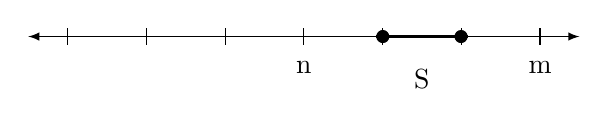
\begin{tikzpicture}

\draw[latex-latex] (-3.5,0) -- (3.5,0) ; %edit here for the axis
\foreach \x in  {-3,-2,-1,0,1,2,3} % edit here for the vertical lines
\draw[shift={(\x,0)},color=black] (0pt,3pt) -- (0pt,-3pt);
\foreach \x in {,,,,,,} % edit here for the numbers
\draw[shift={(\x,0)},color=black] (0pt,0pt) -- (0pt,-3pt) node[below] 
{$\x$};
\draw[*-*] (0.92,0) -- (2.08,0);
\draw[very thick] (0.92,0) -- (2.08,0);

\node [below] at (1.5,-0.3) {S};
\node [below] at (0, -0.2) {n};
\node [below] at (3, -0.2) {m};

\end{tikzpicture}

If an upper bound m of S is a member of S, then m is called the maximum (or largest element) of S, and we say that m = \textbf{max S}.

--n--[--S--m--

Similarly, we may decline \textbf{minimum} of S \textbf{(n = min S)}.

\

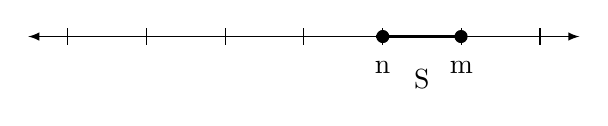
\begin{tikzpicture}

\draw[latex-latex] (-3.5,0) -- (3.5,0) ; %edit here for the axis
\foreach \x in  {-3,-2,-1,0,1,2,3} % edit here for the vertical lines
\draw[shift={(\x,0)},color=black] (0pt,3pt) -- (0pt,-3pt);
\foreach \x in {,,,,,,} % edit here for the numbers
\draw[shift={(\x,0)},color=black] (0pt,0pt) -- (0pt,-3pt) node[below] 
{$\x$};
\draw[*-*] (0.92,0) -- (2.08,0);
\draw[very thick] (0.92,0) -- (1.92,0);

\node [below] at (1.5,-0.3) {S};
\node [below] at (1, -0.2) {n};
\node [below] at (2, -0.2) {m};

\end{tikzpicture}

}

\bsc{Theorem 1}{
If a set S $\sbs \br$ possesses a max element, then it is unique. A similar result holds for a minimum element.
\bgpf
\supp{$\exists m_1, m_2 \in \br$ st $m_1 =$ max S, $m_2 = $ max S}

Thus, $m_1$, $m_2 \in S$ and, $\fa s \in$ S

\step{s \leq m_1}{1}
\step{s \leq m_2}{2}

Let max $=$ \uw{m}{1} in \bpth{1} and max $=$ \uw{m}{2} in \bpth{2} to obtain that \uw{m}{2} $\leq$ \uw{m}{1} and \uw{m}{1} $\leq$ \uw{m}{2}, \

Hence, \uw{m}{1} \eql \uw{m}{2}. 
\epf
}
\bsc{Definition 3.3.5 (supremum defined)}{
Let \es $\neq$ S \sbs \br if S is bounded above, \

then the \textbf{least upper bound} of S is called the \textbf{supremum} of S, denoted by sup S \mem \br \

iff: \

\balist
\item s $\leq$ sup S \fa s \mem S
\item \exs s' \mem S st sup S $-$ \ep $<$ s' \fa \ep $>$ 0
\elist

\ssc{Axiom of Completeness of the set of Real Numbers: \br}{
Every \es $\neq$ S \sbs \br that is bounded above has a least upper bound (i.e. sup S \mem \br exists). \

A similar statement can be made about inf S.
}

Remark: In practice 3.3.4, the set T \eql \{q \mem \bq : $0 \leq q \leq \sqrt{2}$\} is bounded.

\

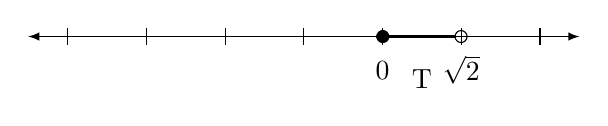
\begin{tikzpicture}

\draw[latex-latex] (-3.5,0) -- (3.5,0) ; %edit here for the axis
\foreach \x in  {-3,-2,-1,0,1,2,3} % edit here for the vertical lines
\draw[shift={(\x,0)},color=black] (0pt,3pt) -- (0pt,-3pt);
\foreach \x in {,,,,,,} % edit here for the numbers
\draw[shift={(\x,0)},color=black] (0pt,0pt) -- (0pt,-3pt) node[below] 
{$\x$};
\draw[*-o] (0.92,0) -- (2.08,0);
\draw[very thick] (0.92,0) -- (1.92,0);

\node [below] at (1.5,-0.3) {T};
\node [below] at (1, -0.2) {$0$};
\node [below] at (2, -0.12) {$\sqrt{2}$};

\end{tikzpicture}

\newpage

But $\sqrt{2}$ is not rational, so the set wouldn't have a least upper bound.

We need to fill in the gaps to make analysis work.
}

\bsc{Examples (\#3, page 132):}{

\balist
\item S \eql \{1, 3\} \

	sup S \eql 3 \lra since s $\leq$ 3 \fa s \mem S and 3 $- \epsilon < 3$
\item similar to a.
\item S \eql (0, 4] \

	sup S \eql 4, max S \eql 4
\item S \eql (0, 4) \

	sup S \eql 4 \lra since s $\leq$ 4 \fa s \mem S and 4 $- \epsilon < s'$ \mem S \
	
	max S = undefined. There is no max.
\item S \eql \{ \frc{1}{2n} : n \mem \bn\} \

	sup S \eql \frc{1}{2} \
	
	max S \eql \frc{1}{2} (if the supremum is in the set, then max \eql sup)
\item S \eql \{ 1 $-$ \frc{1}{2n} : n \mem \bn\} \

	sup S \eql 1 \
	
	max S \eql undefined (1 $\not\in$ \br)

\elist

}

\end{document}